% LIPAS conference poster — portrait A0, two columns, single page
\documentclass[12pt]{article}

\usepackage[paperwidth=841mm,paperheight=1189mm,margin=12mm,top=10mm,bottom=10mm]{geometry}
\usepackage{graphicx}
\usepackage{xcolor}
\usepackage{tikz}
\usetikzlibrary{calc}
\usepackage{tcolorbox}
\tcbuselibrary{skins}
\usepackage{enumitem}
\usepackage{ragged2e}
\usepackage{microtype}
\usepackage{fontspec}
\usepackage{setspace}

\definecolor{LipasDark}{HTML}{0B1220}
\definecolor{LipasPanel}{HTML}{E8EDF3}
\definecolor{LipasPanelEdge}{HTML}{C5D0DC}
\definecolor{LipasTeal}{HTML}{2EC4B6}
\definecolor{LipasTitle}{HTML}{F4F7FB}
\definecolor{LipasMuted}{HTML}{A8B4C4}
\definecolor{LipasBody}{HTML}{1A2433}

\setmainfont{Liberation Sans}[
  BoldFont = Liberation Sans Bold,
  ItalicFont = Liberation Sans Italic,
  BoldItalicFont = Liberation Sans Bold Italic
]

\pagestyle{empty}
\setlength{\parindent}{0pt}
\setlength{\parskip}{0.2em}
\setstretch{1.05}

\newcommand{\BodySize}{28pt}
\newcommand{\BodyLead}{34pt}
\newcommand{\SectionHead}{34pt}
\newcommand{\CaptionSize}{18pt}
\newcommand{\TinyFoot}{12pt}

\tcbset{
  lipasbox/.style={
    enhanced,
    colback=LipasPanel,
    colframe=LipasPanelEdge,
    boxrule=1pt,
    arc=4.5mm,
    left=5mm,right=5mm,top=3.5mm,bottom=3.5mm,
    fontupper=\color{LipasBody}\fontsize{\BodySize}{\BodyLead}\selectfont,
    shadow={1.2mm}{-1.2mm}{0mm}{black!15},
    before skip=1.5mm,
    after skip=2mm
  },
  sectiontitle/.style={
    enhanced,
    colback=LipasDark!92,
    colframe=LipasTeal,
    boxrule=0pt,
    borderline west={2.8mm}{0pt}{LipasTeal},
    arc=2.5mm,
    left=5mm,right=4mm,top=2.2mm,bottom=2.2mm,
    fontupper=\color{LipasTitle}\bfseries\fontsize{\SectionHead}{32pt}\selectfont,
    before skip=1mm,
    after skip=1mm
  }
}

\newcommand{\SectionBox}[1]{\begin{tcolorbox}[sectiontitle,width=\linewidth]#1\end{tcolorbox}}
\newcommand{\ContentBox}[1]{\begin{tcolorbox}[lipasbox,width=\linewidth]#1\end{tcolorbox}}
\newcommand{\FigCap}[1]{{\fontsize{\CaptionSize}{18pt}\selectfont\color{LipasBody!80}\RaggedRight #1\par}}

\begin{document}%
\begin{tikzpicture}[remember picture,overlay]
  \fill[LipasDark] (current page.north west) rectangle (current page.south east);
  \node[anchor=south,inner sep=0] at (current page.south)
    {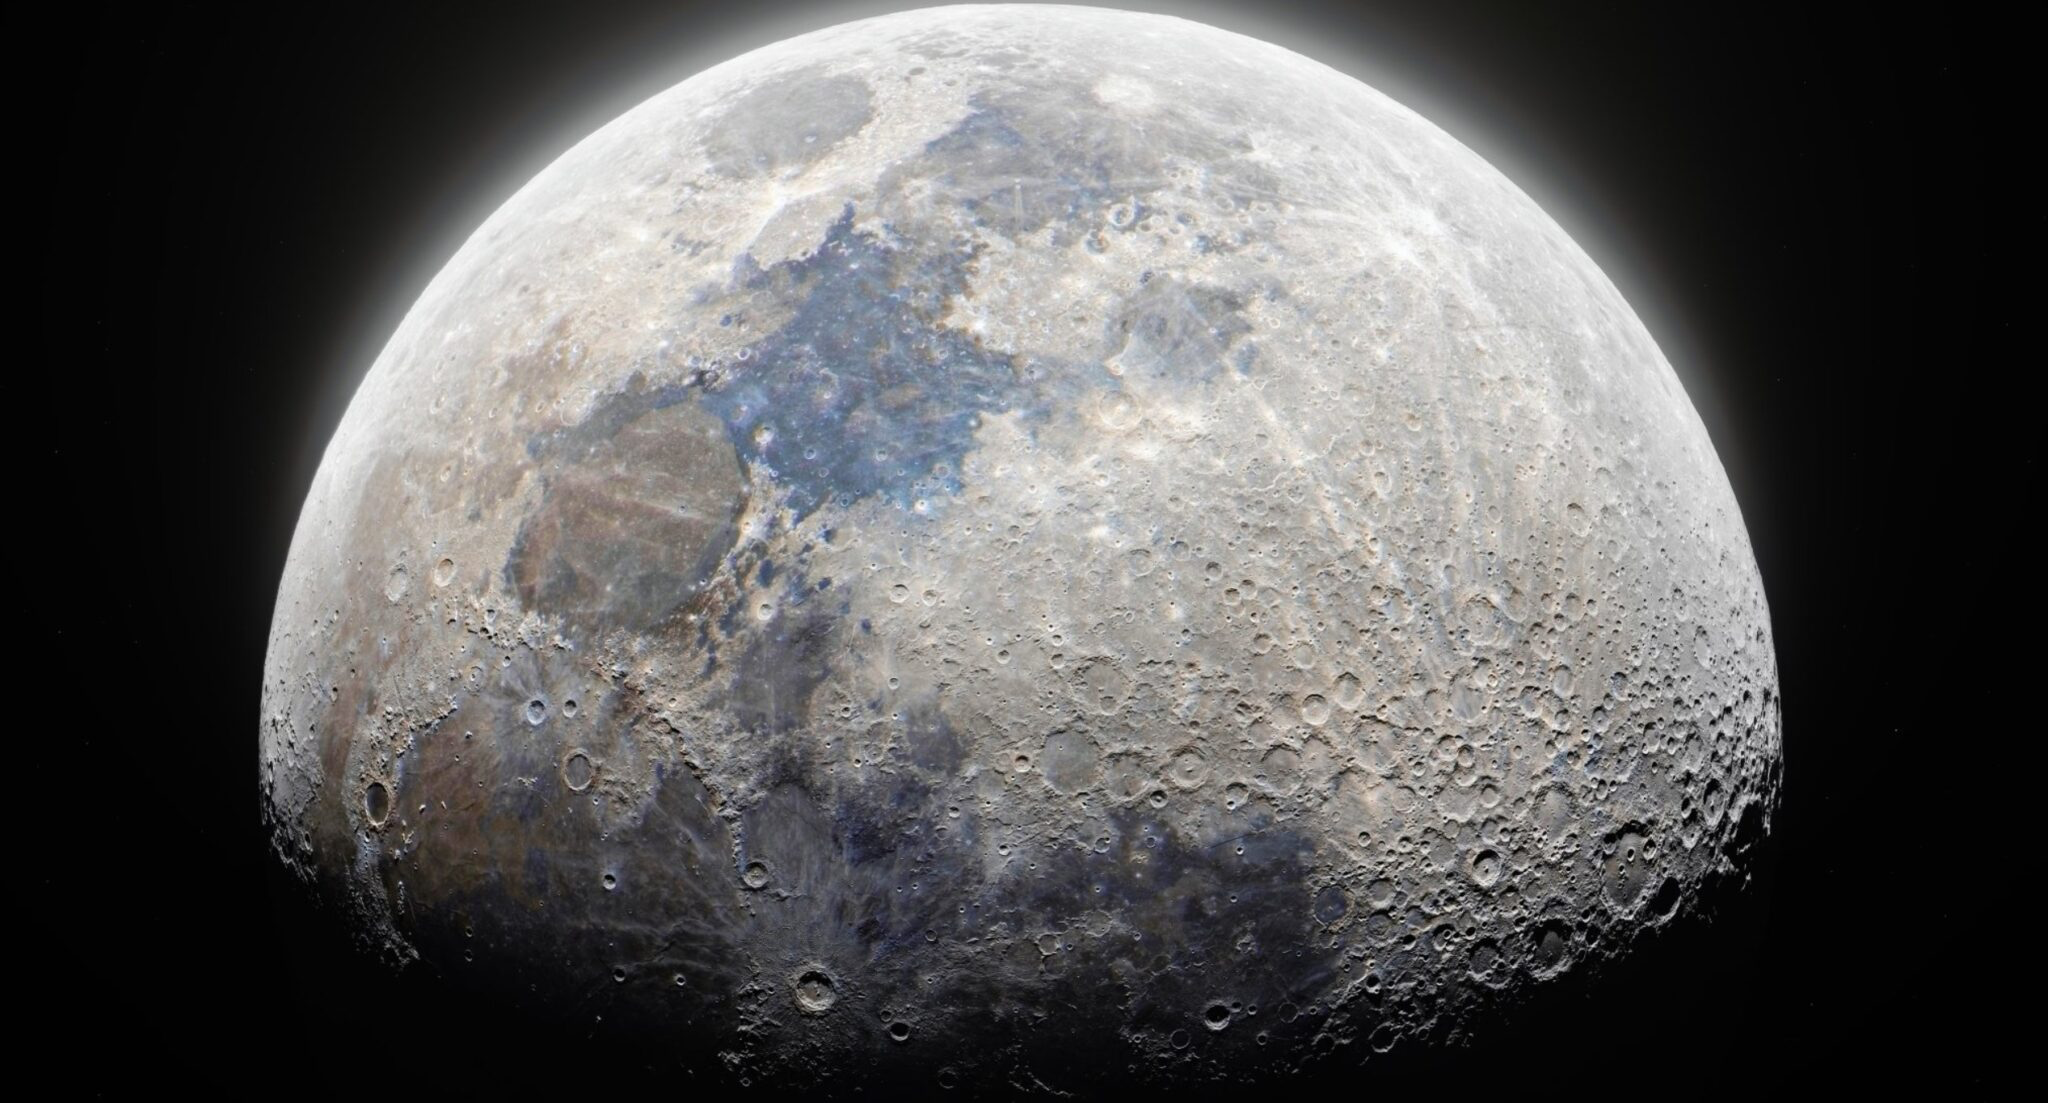
\includegraphics[width=\paperwidth,height=0.42\paperheight,keepaspectratio=false]{assets/moon_bg.png}};
  \fill[LipasDark,opacity=0.62]
    (current page.south west) rectangle ([yshift=0.44\paperheight]current page.south west);
  \node[anchor=south,inner sep=0,opacity=0.9] at ([yshift=52mm]current page.south)
    {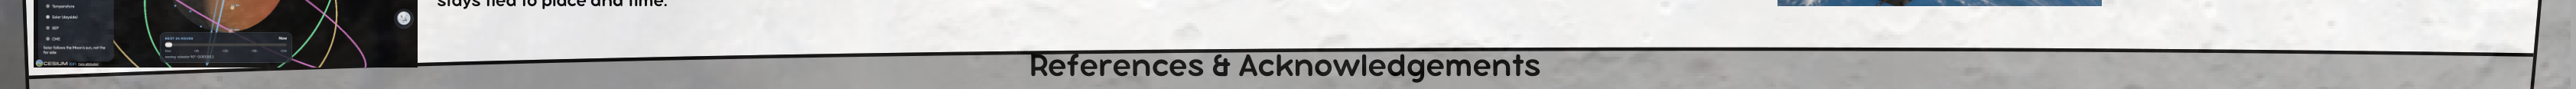
\includegraphics[width=\paperwidth,height=18mm,keepaspectratio=false]{assets/wave_band.png}};
\end{tikzpicture}

\begin{center}
  {\color{LipasTitle}\bfseries\fontsize{50pt}{56pt}\selectfont
  LUNAR IMPACT AND PREDICTIVE ANALYSIS SYSTEM\par}
  \vspace{2mm}
  {\color{LipasTeal}\rule{0.70\textwidth}{1.3mm}\par}
  \vspace{2.5mm}
  {\color{LipasTitle}\fontsize{19pt}{23pt}\selectfont
  Building and Evaluating a Cross Hazard Machine Learning Approach to Unified
  Lunar Forecasting and Mission Planning\par}
  \vspace{2mm}
  {\color{LipasMuted}\fontsize{19pt}{23pt}\selectfont
  Luka Takki \quad$\cdot$\quad Luxembourg 2026\par}
\end{center}

\vspace{2mm}

% Fixed-height two-column stage so content stays on one A0 page
\noindent
\begin{minipage}[t]{0.485\textwidth}
%% ================= LEFT =================
\SectionBox{Abstract}
\ContentBox{%
LIPAS (Lunar Impact and Predictive Analysis System) is a hybrid forecasting and decision-support
platform that combines Long Short-Term Memory (LSTM) machine learning with physics-based
models to predict lunar space weather (temperature, radiation, micrometeorites, and solar
storms). Users can view forecasts for any lunar location on an interactive web dashboard. This
study evaluated whether a system like LIPAS could be developed, whether it was usable, and
whether it could produce accurate forecasts. Results: $\sim$15\% lower solar RMSE and $\sim$22\% lower
radiation RMSE compared with NASA-replicated flagship models, with earlier solar storm EVA
caution alerts than NASA (T+45 vs T+55).
}

\SectionBox{Introduction}
\ContentBox{%
Renewed lunar exploration through initiatives such as NASA's Artemis programme increases the
need for faster and more accurate operational forecasting tools. Existing models often address
individual hazards, requiring mission planners to consult multiple products when making time-
critical decisions. LIPAS addresses this challenge by integrating forecasting approaches into a
single decision-support platform enhanced by machine learning.

\vspace{1mm}
This study addresses three research questions:\\[0.5mm]
RQ1: Can physics and machine learning be combined into an hybrid lunar forecast system?\\
RQ2: Does unifying multiple hazards into one mission platform improve operational usability?\\
RQ3: Can LIPAS improve selected hazard forecasts versus established NASA/NOAA baselines?
}

\SectionBox{System Overview}
\ContentBox{%
\begin{minipage}[t]{0.32\linewidth}
\centering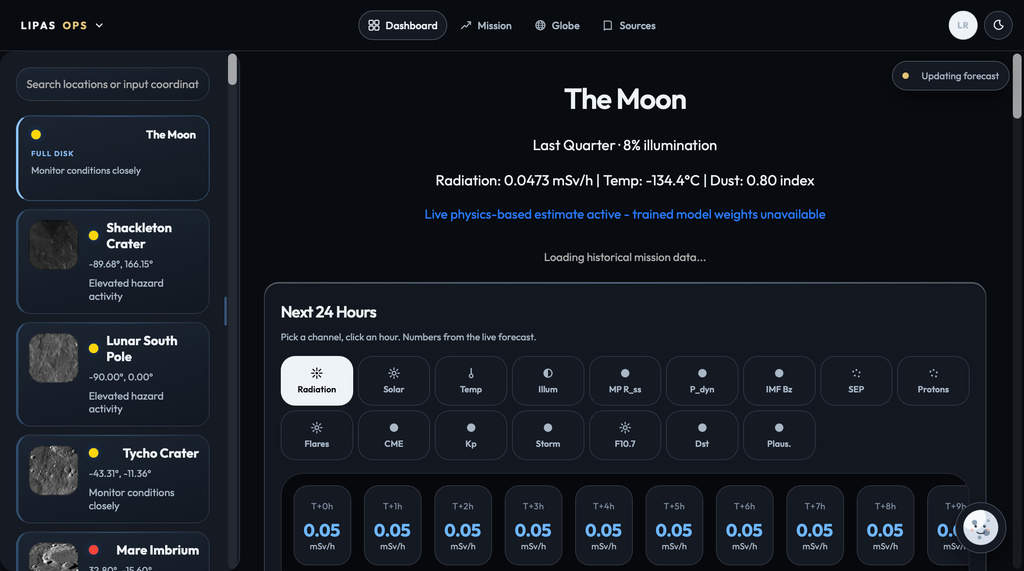
\includegraphics[width=\linewidth,height=115mm,keepaspectratio]{assets/ui_dashboard.png}\\[1mm]
{\bfseries\fontsize{17pt}{21pt}\selectfont Dashboard\par}
{\fontsize{17pt}{21pt}\selectfont\raggedright Live six hazard forecasts, maps, trends, and alerts in one view.\par}
\end{minipage}\hfill
\begin{minipage}[t]{0.32\linewidth}
\centering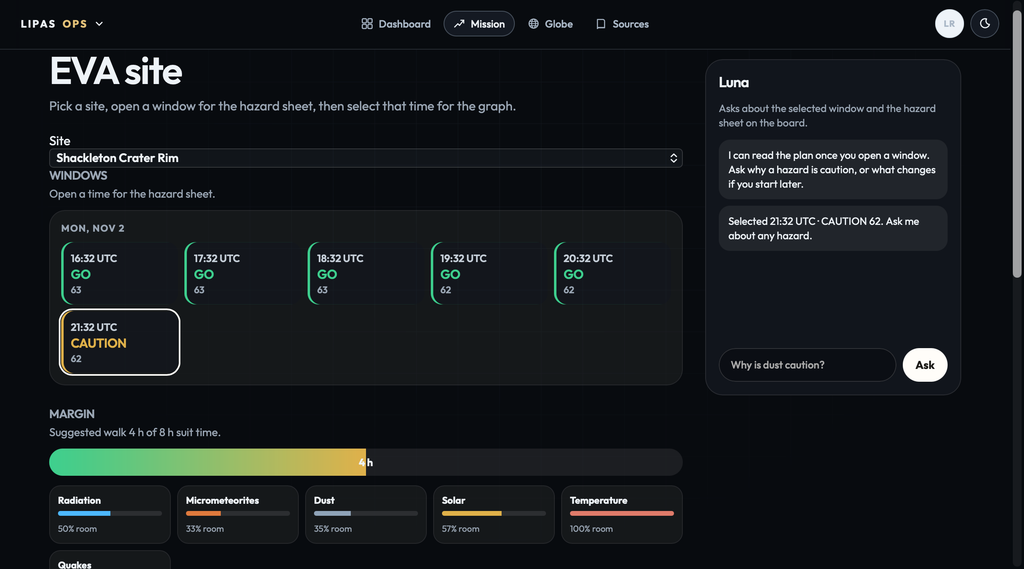
\includegraphics[width=\linewidth,height=115mm,keepaspectratio]{assets/ui_mission.png}\\[1mm]
{\bfseries\fontsize{17pt}{21pt}\selectfont Mission planner\par}
{\fontsize{17pt}{21pt}\selectfont\raggedright Go / caution / no go for an EVA from place and duration.\par}
\end{minipage}\hfill
\begin{minipage}[t]{0.32\linewidth}
\centering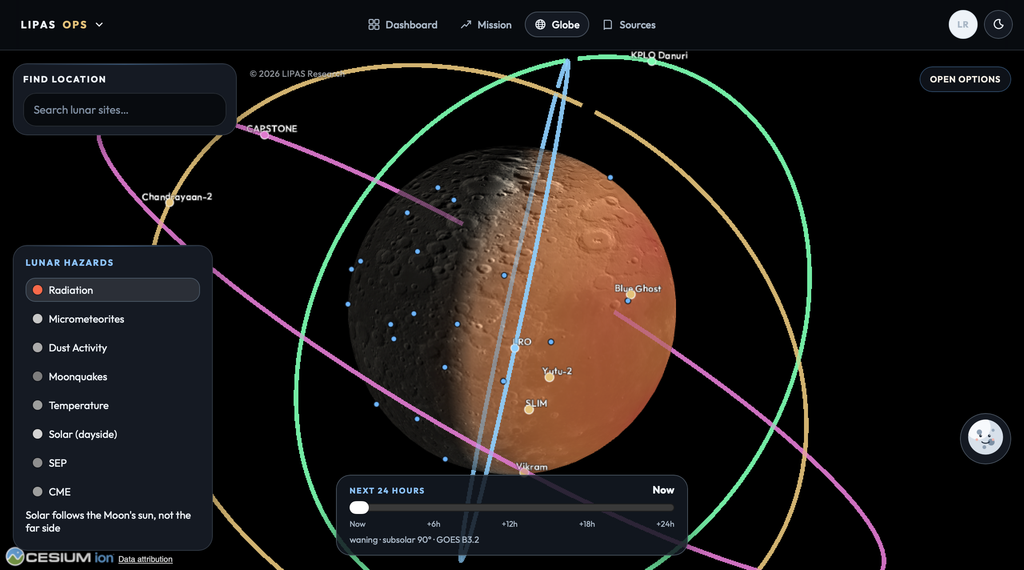
\includegraphics[width=\linewidth,height=115mm,keepaspectratio]{assets/ui_site.png}\\[1mm]
{\bfseries\fontsize{17pt}{21pt}\selectfont Site map\par}
{\fontsize{17pt}{21pt}\selectfont\raggedright Inspect any lunar location with local hybrid forecasts.\par}
\end{minipage}
}

\SectionBox{Methods}
\ContentBox{%
LIPAS forecasts each lunar hazard by joining physics based estimates (agency style NASA and NOAA methods, live APIs, and historical archives) with a temporal LSTM that reads 18 features over a 72 day window. The two streams are blended with locked, hazard specific weights so machine learning corrects channels where it helps and physics leads where the relation is already strong. The formula below states that blend; the flowchart shows the live data path into six hazard outputs. The experimental design used a qualitative ranking against single purpose tools; a quantitative evaluation at three locations (equatorial reference, Apollo 11, and Nobile Rim) across two locked windows (summer Window A, 1 June to 4 August 2026, 195 site days of quiet to mixed space weather; storm Window B, 20 April to 20 May 2024, 93 site days of disturbed drivers) so accuracy could be judged in both quiet and storm regimes; a radiation focused EVA mission simulation for warning time; and a cross hazard input ablation.

\vspace{2mm}
\centering
{\fontsize{28pt}{34pt}\selectfont
$\displaystyle \hat{y}_{t}=w_{1}\,ML_{t}+(1-w_{1})\,Physics_{t}$
\par}
\vspace{1.5mm}
\raggedright
{\fontsize{17pt}{21pt}\selectfont
Here $\hat{y}_{t}$ is the hybrid forecast at time $t$,
$ML_{t}$ is the LSTM output,
$Physics_{t}$ is the physics based estimate, and
$w_{1}$ is the locked machine learning weight for that hazard
(with $1-w_{1}$ the physics share).
\par}
\vspace{2mm}
\centering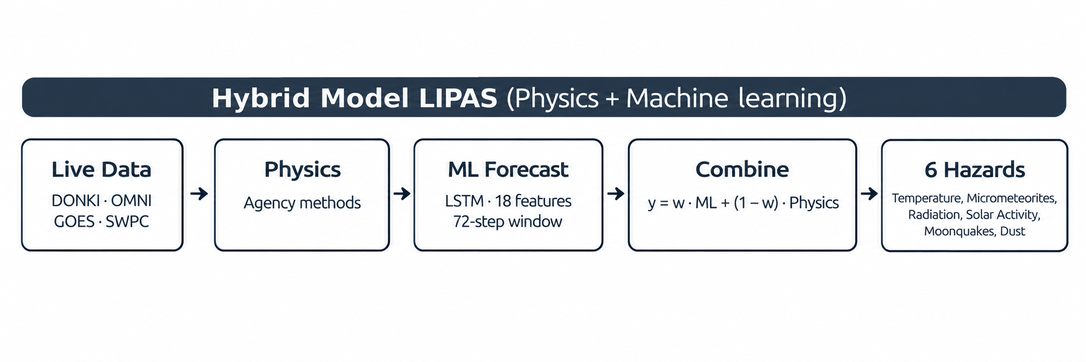
\includegraphics[width=\linewidth,height=130mm,keepaspectratio]{assets/flowchart.png}\\[1.5mm]
\centering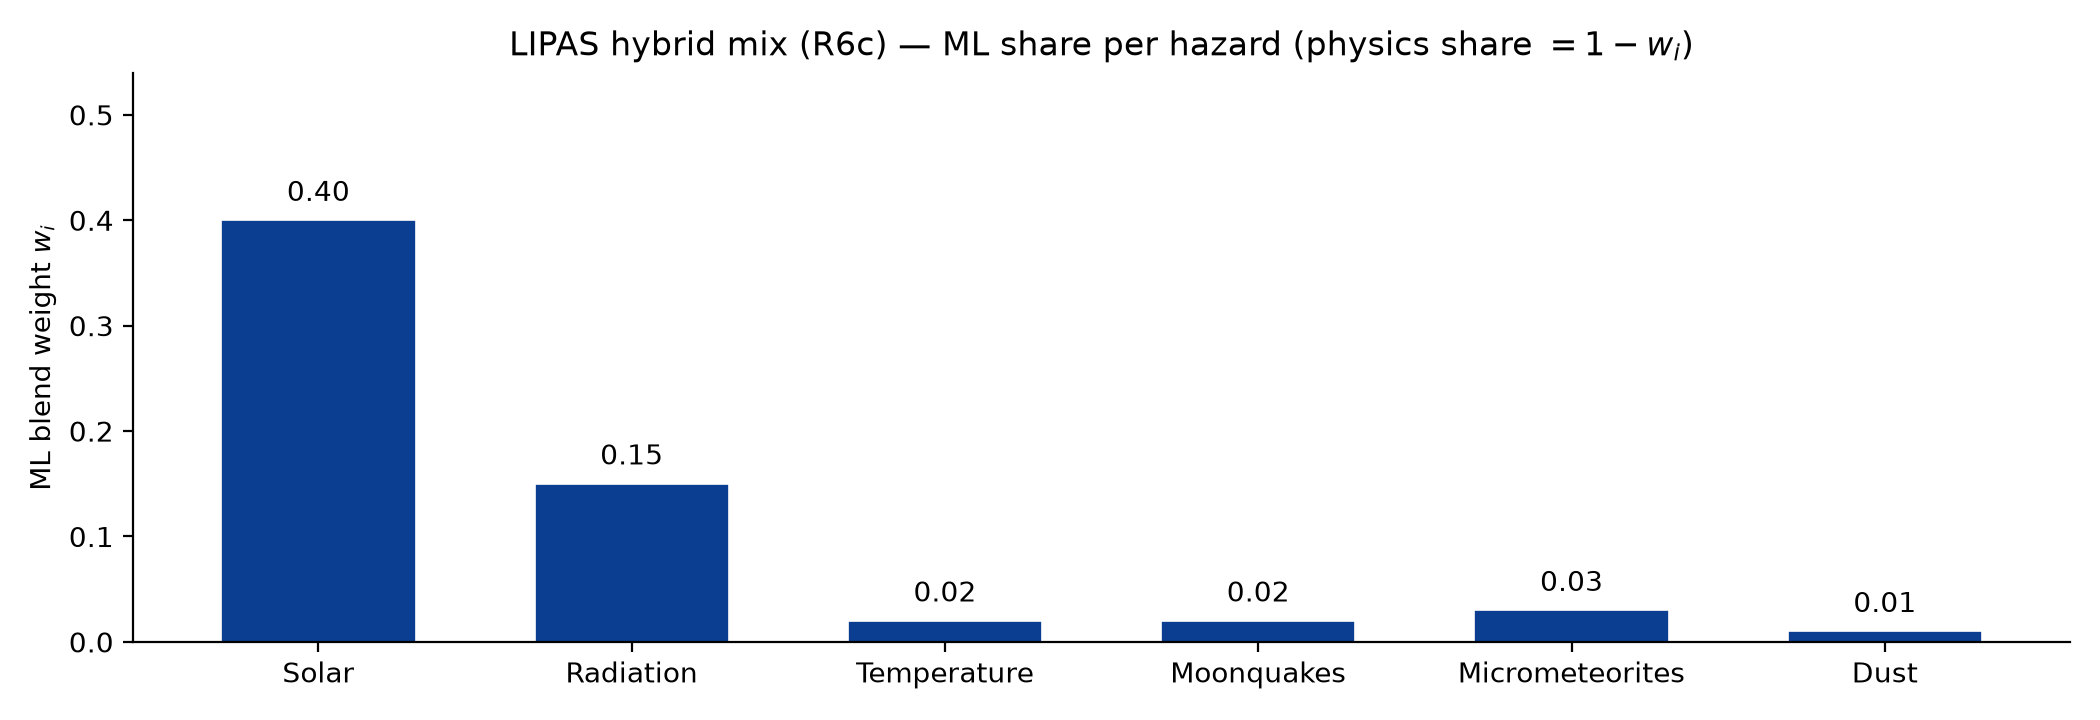
\includegraphics[width=0.92\linewidth,height=75mm,keepaspectratio]{figures/fig_architecture_blend.png}\\[0.5mm]
\FigCap{Locked hybrid mix: solar and radiation keep learned corrections; temperature, moonquakes, micrometeorites, and dust stay mostly physics led.}
}
\end{minipage}%
\hfill
\begin{minipage}[t]{0.485\textwidth}
%% ================= RIGHT =================
\SectionBox{Results}
\ContentBox{%
Across both locked evaluation windows, LIPAS beat the replicated baselines on every hazard while temperature, moonquakes, and dust stayed nearly physics tied. Summer Window A (1 June to 4 August 2026, 195 site days) cut solar RMSE by about 3.6\% and radiation by about 3.7\%. Storm Window B (20 April to 20 May 2024, 93 site days) was the standout: solar improved by about 18.6\% and radiation by about 58.7\%. Micrometeorite gaps looked huge when AMS shower timing was included versus MEM 3 seasonal only, but those labels are circular, so they illustrate shower timing rather than an independent win. In the EVA mission simulation, LIPAS issued caution at T+50, earlier than combined NASA (T+55) and far earlier than GOES only (T+80), and reached no go at T+55 versus GOES T+105, showing the ops value of one unified forecast view.

\vspace{2mm}
{\bfseries\fontsize{19pt}{23pt}\selectfont Window A: four key hazards\par}
\vspace{1mm}
\begin{minipage}[t]{0.485\linewidth}
\centering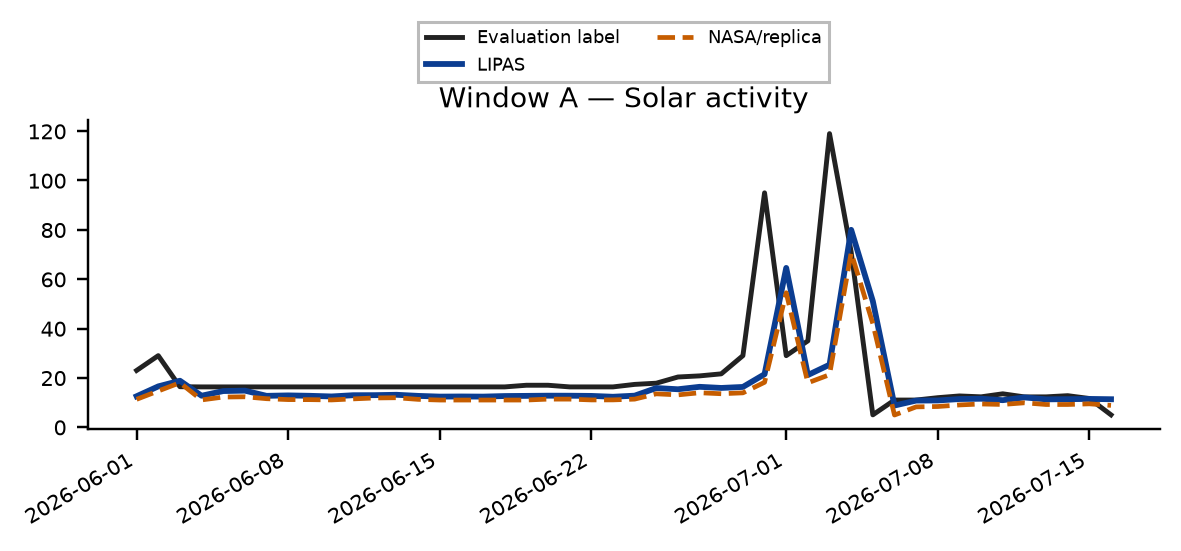
\includegraphics[width=\linewidth,height=105mm,keepaspectratio]{figures/fig_windowA_solar_activity.png}\\
\FigCap{Solar: about 3.6\% lower RMSE.}
\end{minipage}\hfill
\begin{minipage}[t]{0.485\linewidth}
\centering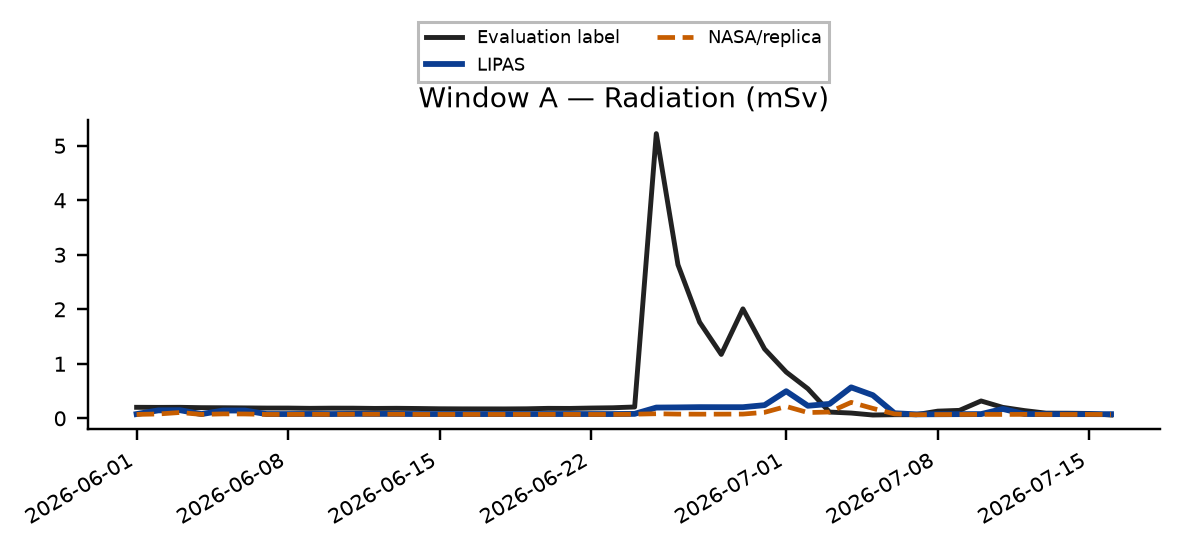
\includegraphics[width=\linewidth,height=105mm,keepaspectratio]{figures/fig_windowA_radiation_mSv.png}\\
\FigCap{Radiation: about 3.7\% lower RMSE.}
\end{minipage}\\[1.5mm]
\begin{minipage}[t]{0.485\linewidth}
\centering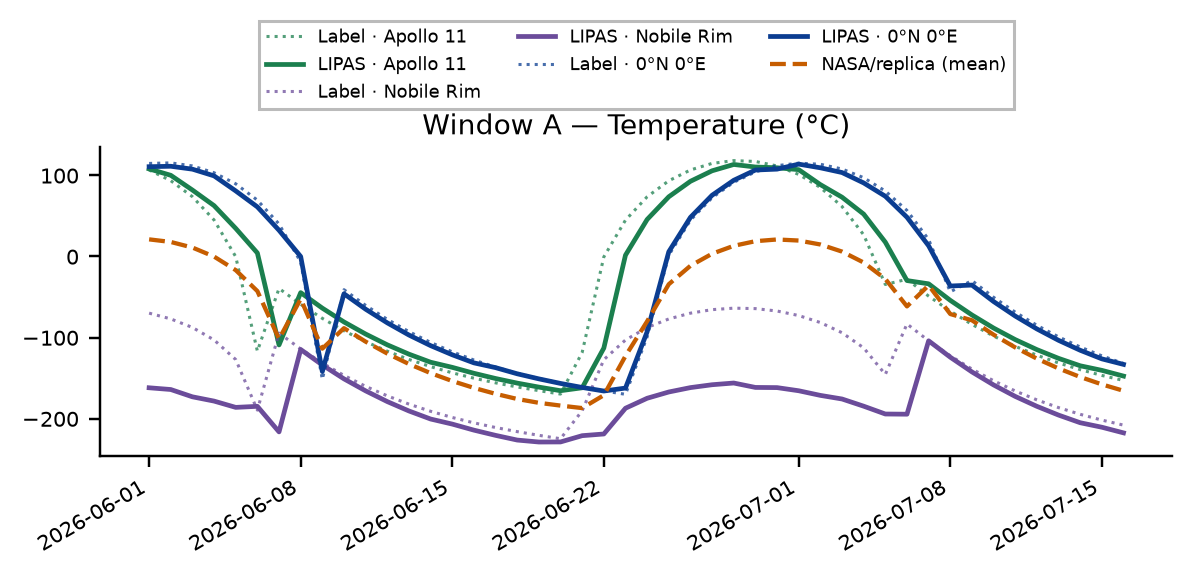
\includegraphics[width=\linewidth,height=105mm,keepaspectratio]{figures/fig_windowA_temperature_C.png}\\
\FigCap{Temperature: three sites where latitude matters.}
\end{minipage}\hfill
\begin{minipage}[t]{0.485\linewidth}
\centering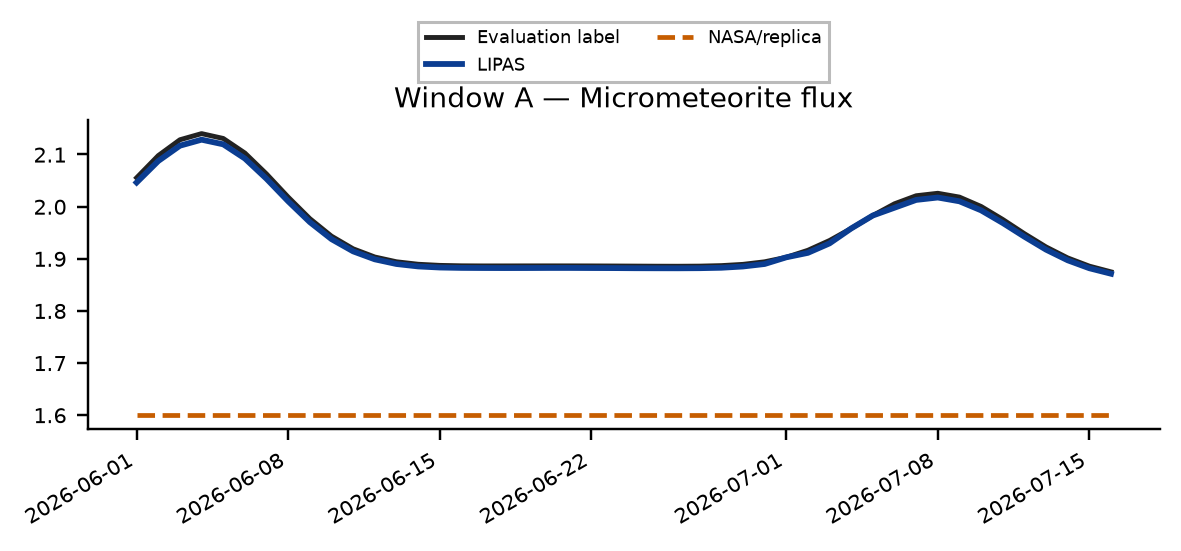
\includegraphics[width=\linewidth,height=105mm,keepaspectratio]{figures/fig_windowA_meteor_flux_1e15.png}\\
\FigCap{Micrometeorites: circular shower timing illustration.}
\end{minipage}

\vspace{2mm}
{\bfseries\fontsize{19pt}{23pt}\selectfont Window B: storm solar and radiation\par}
{\fontsize{17pt}{21pt}\selectfont
Storm Window B stresses space weather drivers. These charts show the clearest hybrid separation: solar RMSE fell by about 18.6\% and radiation by about 58.7\% versus the replicas.
\par}
\vspace{1mm}
\begin{minipage}[t]{0.485\linewidth}
\centering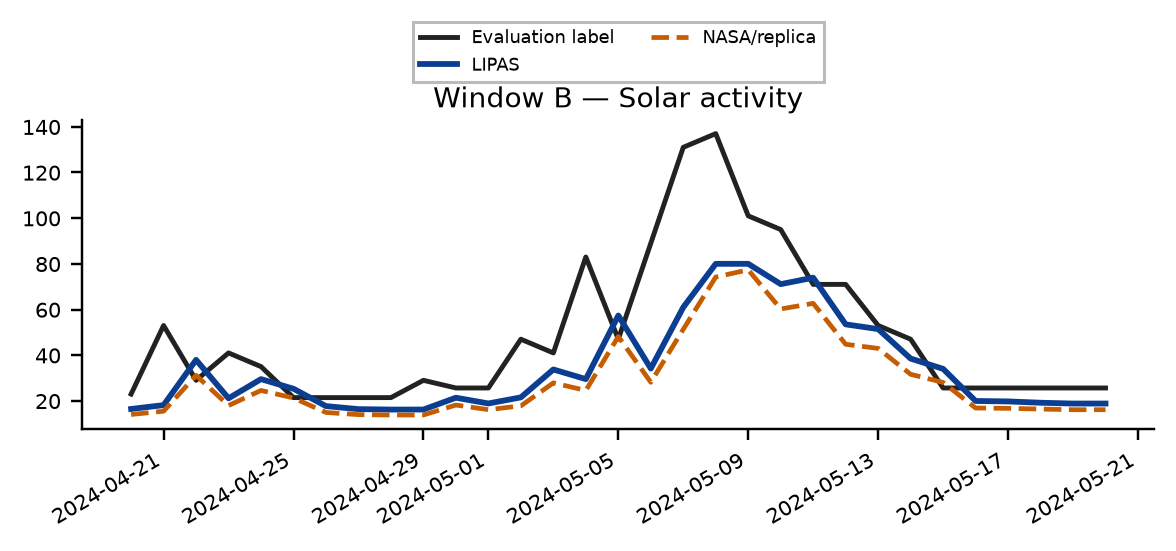
\includegraphics[width=\linewidth,height=95mm,keepaspectratio]{figures/fig_windowB_solar_activity.png}\\
\FigCap{Window B solar: larger hybrid margin when disturbed.}
\end{minipage}\hfill
\begin{minipage}[t]{0.485\linewidth}
\centering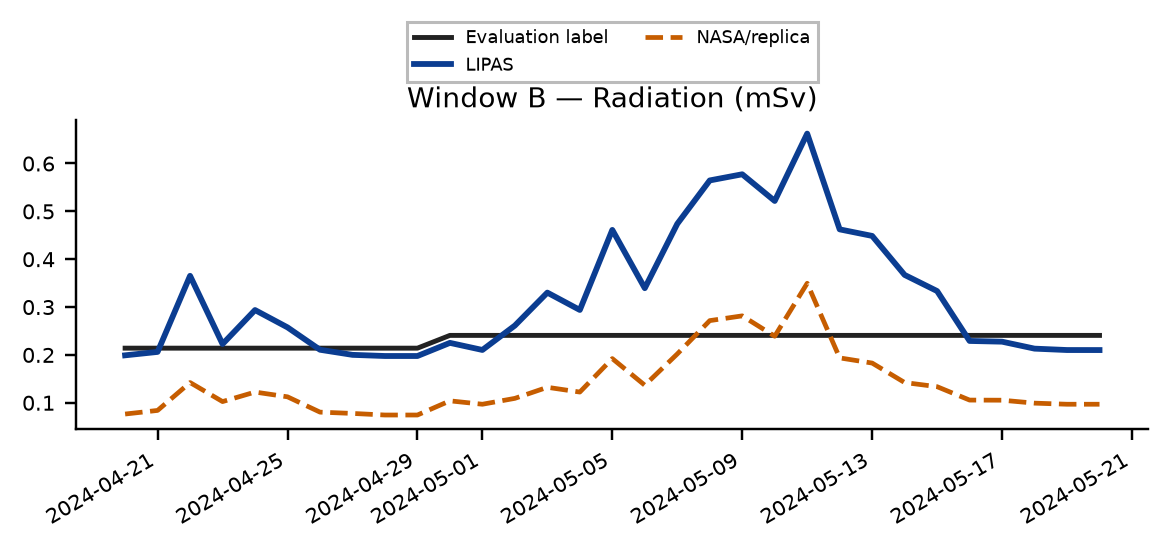
\includegraphics[width=\linewidth,height=95mm,keepaspectratio]{figures/fig_windowB_radiation_mSv.png}\\
\FigCap{Window B radiation: strongest locked accuracy gain.}
\end{minipage}

\vspace{2mm}
{\bfseries\fontsize{19pt}{23pt}\selectfont Mission simulation\par}
{\fontsize{17pt}{21pt}\selectfont
Apollo length EVA with a shared radiation script. LIPAS caution T+50 / no go T+55; combined NASA T+55 / T+70; GOES only T+80 / T+105.
\par}
\vspace{1mm}
\centering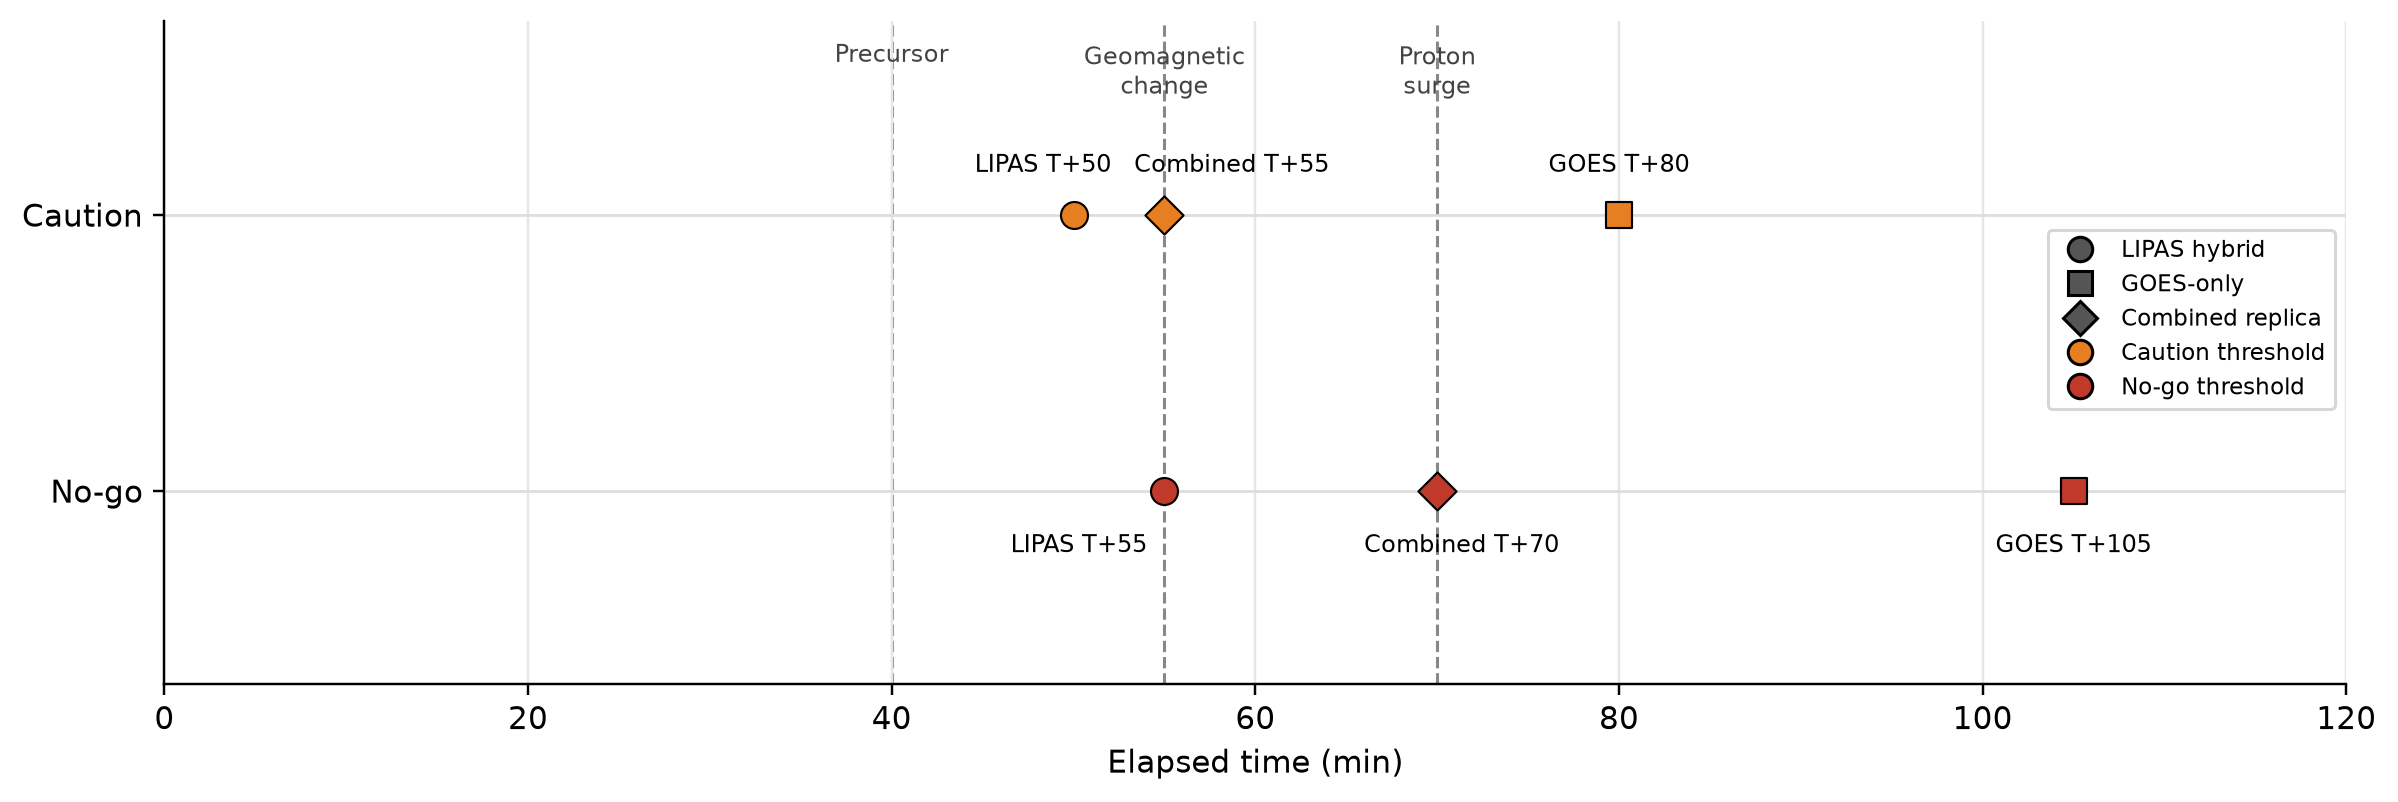
\includegraphics[width=\linewidth,height=115mm,keepaspectratio]{figures/fig_mission_timeline.png}\\[0.5mm]
\FigCap{Earlier unified warnings from upstream solar and geomagnetic drivers, not proton flux alone.}
}

\SectionBox{Discussion and Conclusion}
\ContentBox{%
This study advances a working hybrid lunar forecast stack that joins machine learning with physics in one decision support platform rather than leaving planners to stitch single hazard products by hand.

\vspace{1mm}
\noindent\textbf{RQ1.} Physics and machine learning can be combined into one lunar forecast system: locked blend weights, a 72 day LSTM trunk, and six hazard outputs were built, served, and evaluated end to end.

\vspace{1mm}
\noindent\textbf{RQ2.} Unifying hazards improved operational usability. Qualitative ranking favoured the single view for planning, and the EVA simulation showed LIPAS flagging rising radiation earlier (caution T+50, no go T+55) than combined NASA (T+55 / T+70) and GOES only (T+80 / T+105), while specialised NASA tools still lead on scientific depth.

\vspace{1mm}
\noindent\textbf{RQ3.} Selected accuracy gains versus replicated baselines were real and larger in storm conditions: Window A cut solar and radiation RMSE by about 3.6\% and 3.7\%; Window B improved them by about 18.6\% and 58.7\%. Temperature, moonquakes, and dust stayed nearly physics tied. Micrometeorite gaps that use AMS shower timing are circular illustrations, not independent forecast wins.

\vspace{1.5mm}
LIPAS stands as a research grade decision support layer for lunar planners. It should not make crew decisions without human input, and further validation is required before it could serve as a complete mission control system.
}
\end{minipage}

\vspace{3mm}

\noindent
\begin{tcolorbox}[
  enhanced,
  colback=LipasDark!88,
  colframe=LipasTeal,
  boxrule=0.7pt,
  arc=3mm,
  left=4mm,right=4mm,top=2.5mm,bottom=2.5mm,
  fontupper=\color{LipasTitle}\fontsize{\TinyFoot}{14.5pt}\selectfont,
  width=\linewidth
]
{\bfseries\fontsize{15pt}{18pt}\selectfont References and Acknowledgements\par}
\vspace{1mm}
\begin{minipage}[t]{0.485\linewidth}
{\bfseries SOURCES USED:}\\
NASA DONKI API: https://api.nasa.gov/DONKI/, NOAA SWPC (GOES protons, X ray, Kp):
https://services.swpc.noaa.gov/, NASA OMNI2 Solar Wind Database: https://omniweb.gsfc.nasa.gov, NASA MEM3
Meteoroid Model: https://www.nasa.gov/mem, LADEE LDEX Dust Data: https://pds.nasa.gov/ds-view/pds/viewProfile.jsp?dsid=LADEE-LDEX, Apollo PSE Seismic Catalog: https://pds-geosciences.wustl.edu/missions/apollo/seismic.htm, LRO CRaTER Radiation Products: https://crater-web.sr.unh.edu
\end{minipage}\hfill
\begin{minipage}[t]{0.485\linewidth}
{\bfseries BIG THANKS TO:}\\
Kyle Kennedy, my mentor, for his rigorous evaluation and redesign of methods, studies and the system\\
Prof. Minna Palmroth \& Prof. Emilia Kilpua for their support and guidance at the University of Helsinki\\
Dr. Simon Good for his help in editing the research paper, and providing valuable guidance\\
Dr. Marjo Lipponen-Mraz for her continuous support throughout the European Schools Science Symposium\\
Benjamin Irani-Fey for his coding support during the Nasa Space Apps Challenge
\end{minipage}
\end{tcolorbox}

\end{document}
